\section{Cross-Variable Correlations by Stratum (Q7)}\label{sec:strata_cross}

Grid operations require understanding whether cross-variable relationships are invariant or if they shift across environmental strata. Where cross-variable error correlations exhibit dramatically different trends across day/night, seasonal, or regional classifications, a static, blanket model will systematically misestimate errors.

\subsection{Methods}
To evaluate this stability, we sorted the dataset across four critical axes: time of day, seasons, PJM geographic transmission zones (subset of 9), and individual calendar years (2022-2024). Each of these were then split further into separate day/night matrices based on a \SI{20.0}{W/m^2} GHI threshold.
\raggedbottom
\footnote{Separating the dataset by diurnal phase prevents the severe artificial inflation of correlation coefficients that occurs when blending fundamentally distinct atmospheric processes. For instance, wind-speed errors and temperature errors follow entirely different thermodynamic pathways during the day than they do under a nighttime inversion. GHI gating at \SI{20.0}{W/m^2} is utilized rather than hard-coded clock hours because it naturally adapts to seasonal shifts in daylight length (e.g., summer vs. winter), ensuring that the 'daytime' classification always aligns with actual solar irradiance rather than an arbitrary schedule. }
\flushbottom

With this stratified dataset, we constructed Pearson correlation matrices using the raw forecast errors to quantify the strength and direction of the linear dependencies between variable pairs. Because the Pearson coefficient ($r$) is standardized, it inherently accounts for disparate physical units, such as degrees Celsius for temperature and millibars for pressure. A high positive coefficient indicates a strong, direct linear relationship, while a value near zero suggests no linear association. Conversely, a strongly negative coefficient denotes an inverse linear relationship, wherein an overestimate in one variable's error systematically corresponds to an underestimate in another.
\raggedbottom
\footnote{A key limitation of this approach is that Pearson’s correlation only captures linear associations; any complex, non-linear physical dependencies or thresholds between error vectors remain unquantified by this metric.}
\flushbottom


\subsection{Day/Night Cycle Variations}
The most pronounced differences in error correlations occur across the diurnal cycle, driven by distinct variations in wind, solar forcing, and convective regimes between day and night. Figure~\ref{fig:cross_variable_diurnal_main} illustrates the evolution of the cross-variable Pearson correlation matrix across key diurnal lead times for Forecast Day 1.


The coupling between thermodynamic variables is highly sensitive to solar forcing. The negative correlation between temperature errors and relative humidity errors is a dominant feature across all strata, yet its intensity varies diurnally. At Forecast Hour 06 (\texttt{12:00 UTC / 7:00 EST}, corresponding to early morning), the correlation stands at $r = -0.44$. By Forecast Hour 12 (\texttt{18:00 UTC / 13:00 EST}, afternoon high solar activity), this coupling tightens significantly to $r = -0.72$. Physically, this intensification is consistent with strong daytime heating, where rising afternoon temperatures likely become the primary driver of relative humidity drops

Concurrently, GHI error coupling emerges exclusively during daytime hours. At solar noon, approximately Forecast Hour 12 for the PJM regions (\texttt{18:00 UTC / 13:00 EST}), GHI errors exhibit a notable positive correlation with temperature errors ($r = 0.42$) and a corresponding negative correlation with relative humidity errors ($r = -0.25$). This behavior aligns with a prominent potential model signature: if the HRRR model under-predicts cloud cover, it would over-predict surface GHI, which could drive artificial positive spikes in temperature and dry biases in humidity. At night, around Forecast Hour 24 (\texttt{06:00 UTC / 01:00 EST}), the GHI error row drops entirely to zero due to the absence of solar irradiance, thereby uncoupling the remaining GHI connections.


\begin{figure}[H]
  \centering
  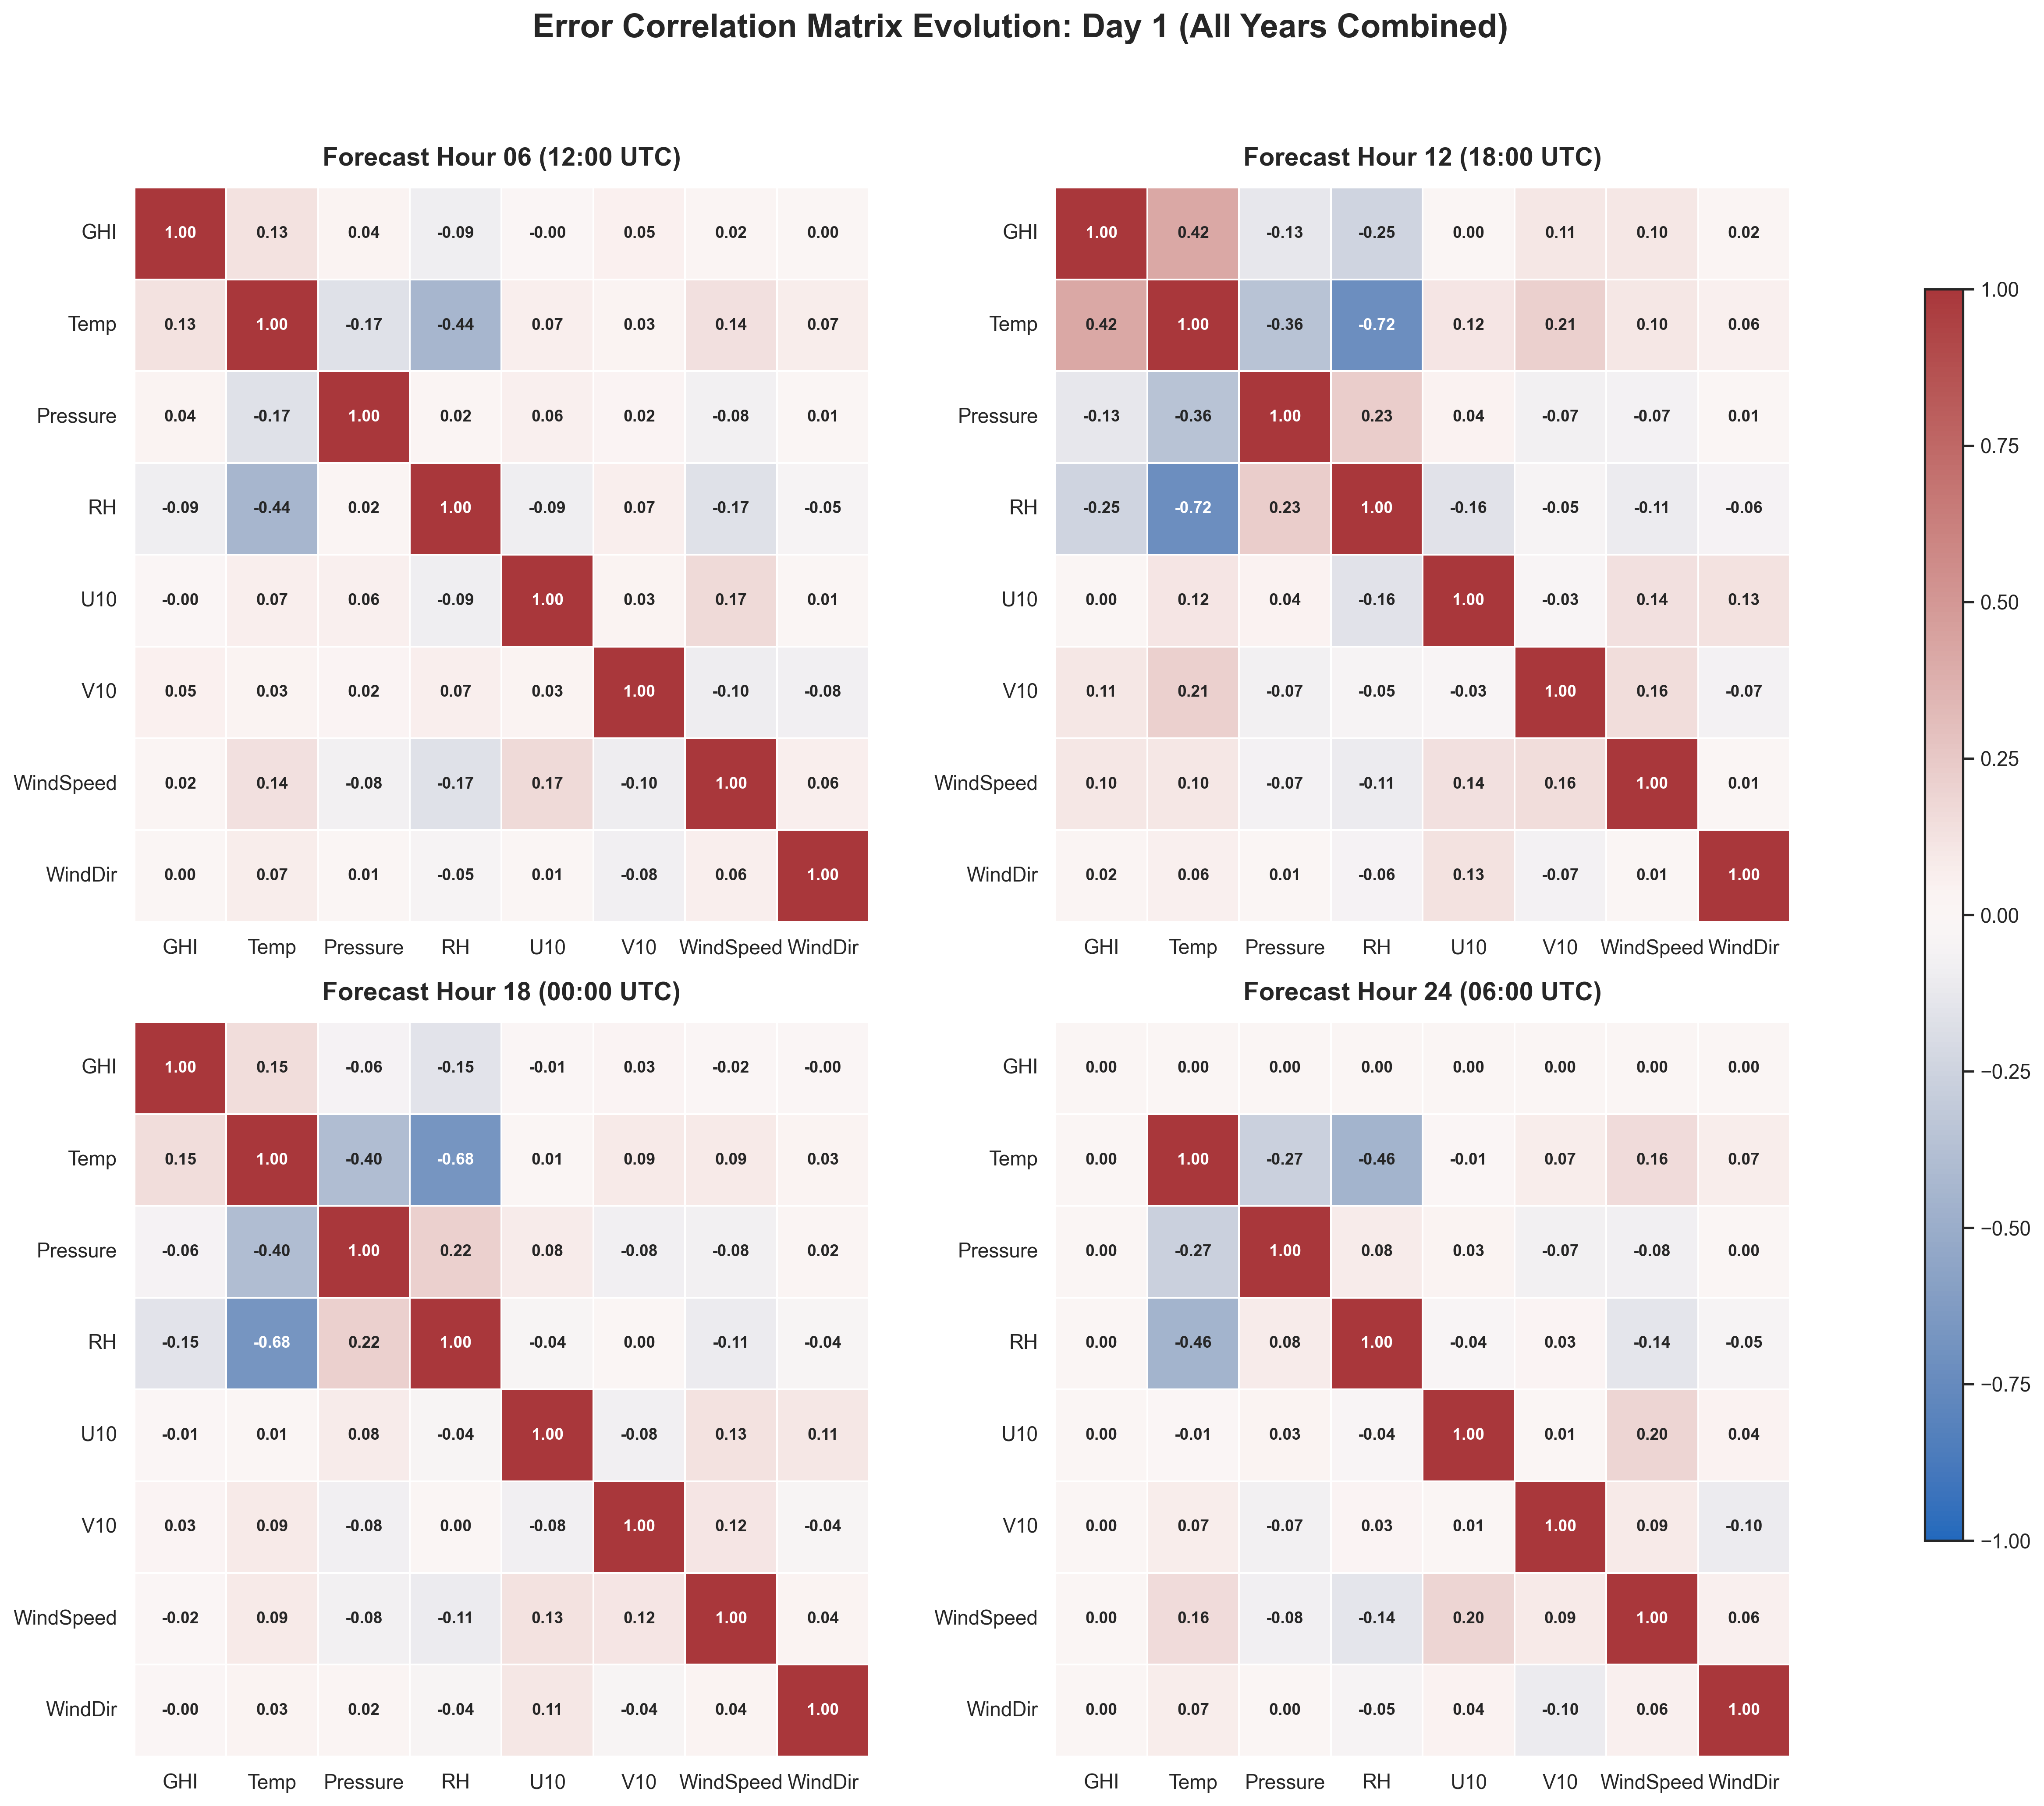
\includegraphics[width=\textwidth]{figures/Q7/TIMEOFDAY/all_variables_corr_day1_horizons.png}
  \caption{Faceted evolution of the cross-variable error Pearson correlation matrix at distinct forecast lead increments (Hours 06, 12, 18, and 24) across Forecast Day 1. The color bar indicates the Pearson $r$ value. The thermodynamic $T/\text{RH}$ coupling intensifies at solar noon (\texttt{18:00 UTC}), while daytime solar-noon GHI errors demonstrate strong phase-locked coupling with thermodynamic variables ($r_{\text{GHI}, T} = 0.42$, $r_{\text{GHI}, \text{RH}} = -0.25$) that completely evaporates at night.}
  \label{fig:cross_variable_diurnal_main}
\end{figure}

\subsection{Seasonal Variations}

In contrast to the rapid shifts observed within the diurnal cycle, the cross-variable error structures exhibit broad consistency across seasons, though specific thermodynamic couplings still experience notable variations. Seasonal matrices for Fall (Figure~\ref{fig:app_fall_day_night}), Spring (Figure~\ref{fig:app_spring_day_night}), Summer (Figure~\ref{fig:app_summer_day_night}), and Winter (Figure~\ref{fig:app_winter_day_night}) reveal that while the foundational structure of the errors remain similar, the intensity of these relationships changes with the seasonal solar and thermal cycle.

The most prominent seasonal difference occurs within the core thermodynamic temperature and relative humidity coupling. This inverse linear relationship is highly sensitive to seasonal characteristics:
\begin{itemize}
    \item \textbf{Summer (Figure~\ref{fig:app_summer_day_night}):} Features the most intense coupling, with daylight $T/\text{RH}$ error correlations reaching $r = -0.80$ and nighttime values at $r = -0.63$, potentially driven by high moisture and hotter surface heating.
    \item \textbf{Spring and Fall (Figure~\ref{fig:app_spring_day_night}, Figure~\ref{fig:app_fall_day_night}):} Display intermediate, nearly identical structural baselines, with Temperature / Relative Humidity (T/RH) couplings holding steady at $r = -0.69$ and $r = -0.68$, respectively. Night hours similarly do not drastically differ between Spring and Fall, with (T/RH) at $r = -0.54$ and $r = -0.52$, respectively.
    \item \textbf{Winter (Figure~\ref{fig:app_winter_day_night}):} Experiences a significant loss in intensity of this coupling, dropping to a daylight low of $r = -0.51$ and a nighttime low of $r = -0.33$. This suppression points to the diminished role of temperature-driven moisture variations during cold, low humidity winter regimes.
\end{itemize}

Secondary variations emerge within the pressure-thermodynamic vectors. In the Summer matrix (Figure~\ref{fig:app_summer_day_night}), temperature and surface pressure errors are moderately coupled during the day ($r = -0.44$), matching a corresponding positive pressure-to-RH error link ($r = 0.32$). In the Winter matrix (Figure~\ref{fig:app_winter_day_night}), however, this pressure-temperature vector weakens to $r = -0.33$, while the pressure-to-RH error link collapses entirely to $r = 0.09$ across both diurnal phases.

Conversely, daylight GHI-to-temperature error links remain remarkably stable across all matrices, fluctuating narrowly between a winter low of $r = 0.29$ (Figure~\ref{fig:app_winter_day_night}) and a spring high of $r = 0.38$ (Figure~\ref{fig:app_spring_day_night}). Wind variables (U10, V10, and Wind Speed) similarly preserve low, decoupled baseline correlations with thermodynamic vectors regardless of the season, indicating that the core spatial wind-prediction error structures remain disconnected from seasonal differences.

\subsection{Interannual Stability}

Year-to-year evaluations across 2022 (Figure~\ref{fig:app_corr_2022}), 2023 (Figure~\ref{fig:app_corr_2023}), and 2024 (Figure~\ref{fig:app_corr_2024}) reveal near-absolute statistical invariance in the cross-variable error structures. Core driving vectors exhibit virtually no annual fluctuations; for instance, the dominant daytime temperature and relative humidity ($T/\text{RH}$) error correlation remains locked between $r = -0.69$ and $r = -0.71$, while the nighttime tracking stays bound tightly between $r = -0.49$ and $r = -0.51$ across all three years. Similarly, secondary daylight links—such as the GHI-to-temperature coupling ($r \approx 0.31$ to $0.35$) and the inverse pressure-to-temperature coupling ($r \approx -0.28$ to $-0.33$)—remain structurally constant. This long-term stability demonstrates that multi-variable error distributions are insulated from yearly model drift.


\subsection{Regional and Zonal Variations}

When evaluated across the individual PJM geographic transmission zones—APS (Figure~\ref{fig:app_zone_aps}), ATSI (Figure~\ref{fig:app_zone_atsi}), COMD (Figure~\ref{fig:app_zone_comd}), DOM (Figure~\ref{fig:app_zone_dom}), EMAC (Figure~\ref{fig:app_zone_emac}), PENE (Figure~\ref{fig:app_zone_pene}), SMAC (Figure~\ref{fig:app_zone_smac}), West (Figure~\ref{fig:app_zone_west}), and WMAC (Figure~\ref{fig:app_zone_wmac})—the cross-variable error matrices exhibit notable spatial uniformity across the core Eastern Interconnection clusters, with a single distinct exception.

For the eight geographically connected eastern and mid-Atlantic zones (spanning from Indianas border through Ohio, Pennsylvania, Maryland, and Virginia...), the baseline error couplings remain closely bounded. Across these eastern footprints, daylight $T/\text{RH}$ stays highly stable within a narrow range ($r \approx -0.69$ to $-0.74$), while daytime GHI to Temperature error links consistently hover between $r = 0.31$ and $r = 0.34$.

The singular structural anomaly emerges within the Commonwealth Edison (COMD) zone matrix (Figure~\ref{fig:app_zone_comd}). Situated in northern Illinois, COMD sits at the far northwestern fringe of the PJM territory, geographically isolated from the dense eastern coastal cluster. In the COMD daylight matrix, the characteristic $T/\text{RH}$ inverse error correlation weakens significantly to $r = -0.64$, while the daytime pressure-to-temperature coupling attenuates to $r = -0.29$ compared to the fleet baseline (such as $r = -0.38$ in DOM).

This localized divergence points towards a climate transition: while the eastern assets are bound to uniform, ocean-influenced or rolling Appalachian air masses, COMD’s boundary-layer errors are governed by the drier, more volatile continental climates of the upper Midwest. This localized shift suggests that while regional error profiles are largely static across the eastern footprint, far-western grid expansions introduce microclimate boundary conditions that require highly-localized joint error calibration.



\subsection{Findings and Implications}

The evaluation of the HRRR cross-variable error matrices reveals clear boundaries between highly dynamic weather factors and static, predictable baselines. These insights outline when and where joint error modeling matters most.

\begin{itemize}
    \item \textbf{Dominant Diurnal and Regional Drivers:} The most severe structural changes occur across the day/night cycle and at extreme geographic boundaries. Diurnal shifts alter the entire thermodynamic framework, creating complex error couplings (such as daytime GHI/T $r= 0.42$) that completely uncouple at night. Regionally, while error profiles are stable across the contiguous eastern PJM footprint, far-western zones like COMD introduce distinct microclimatic shifts that require localized joint calibrations.
    \item \textbf{Moderate Seasonal Scaling:} Seasonal transitions act as a scaling factor rather than a structural change. The fundamental orientation of the matrices remains intact, but the intensity of core thermodynamic variables differs alongside seasonal  humidity, peaking in Summer (T/RH $r = -0.80$) and dropping in Winter ( T/RH $r = -0.51$).
    \item \textbf{Negligible Interannual Drift:} Year-to-year cross-variable error distributions across 2022, 2023, and 2024 exhibit nearly absolute statistical invariance. This stability suggests that joint distributions looking at multi-year historical datasets remain highly reliable for forward-looking scheduling.
\end{itemize}

A key operational limitation of this framework is its reliance on Pearson correlation, which exclusively captures linear associations. Complex, non-linear physical thresholds between error vectors—such as an error in one variable triggering an order-of-magnitude leap in another—remain unquantified by this metric. Future iterations of this risk-modeling framework could leverage non-linear regression techniques or copula-based joint distributions to more accurately map threshold-dependent error behavior under extreme grid scenarios.
